\documentclass{standalone}
\usepackage{tikz}
\usetikzlibrary{shapes}
\usepackage{tikzpeople}

\begin{document}
			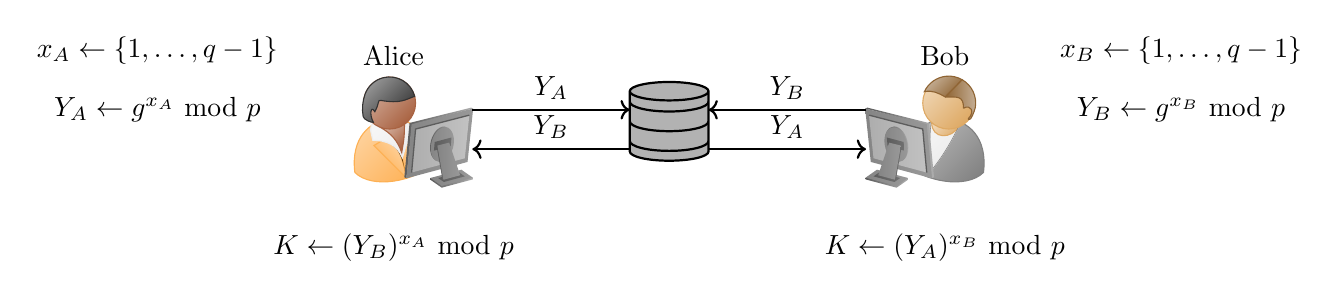
\begin{tikzpicture}
				\tikzset{database/.style={
						cylinder,
						aspect=1,
						draw,
						thick,
						fill,
						shape border rotate=90,
						minimum height=1cm,
						left color=black!30,
						right color=black!30,
						middle color=black!30,
						minimum width=1cm,
						path picture={
							\draw[black, thick] let \p1=($(path picture bounding box.north east)-(path picture bounding
							box.south west)$) in
							foreach \XX in {1,2,3}  {([yshift=-\XX*\y1/4]path picture bounding box.north west)
								arc(180:360:\x1/2 and 0.25*\x1/2)};
				}}}
				
				
				%% DELIVERY SERVER
				\node[database] (DB1) at (3.5,0) {};
				\node[alice, monitor, label=Alice, minimum size=1cm] (Alice) at (0,0) {};
				\node[bob, mirrored, monitor, label=Bob, minimum size=1cm] (Bob) at (7,0) {};
				
				\draw[->, thick] (1,0.25)  -- (3,0.25) node[midway, above] {$Y_A$};
				\draw[->, thick] (6,0.25)  -- (4,0.25) node[midway, above] {${Y_B}$};
				\draw[<-, thick] (1,-0.25)  -- (3,-0.25) node[midway, above] {${Y_B}$};
				\draw[<-, thick] (6,-0.25)  -- (4,-0.25) node[midway, above] {${Y_A}$};
				
				\node[] (AGen) at (-3,1) {${x_A} \gets \{1,\ldots,q-1\}$};
				\node[] (AEncap) at (-3,0.25) {${Y_A} \gets g^{{x_A}}$ mod $p$};
				\node[] (ADecap) at (0,-1.5) {${K} \gets ({Y_B})^{{x_A}}$ mod $p$};
				\node[] (BGen) at (10,1) {${x_B} \gets \{1,\ldots,q-1\}$};
				\node[] (BEncap) at (10,0.25) {${Y_B} \gets g^{{x_B}}$ mod $p$};
				\node[] (BDecap) at (7,-1.5) {${K} \gets ({Y_A})^{{x_B}}$ mod $p$};
				
			\end{tikzpicture}

\end{document}
